\chapter{Исследовательская часть}

\section{Технические характеристики}

Технические характеристики устройства, на котором выполнялось тестирование:

\begin{itemize}
	\item Операционная система: Ubuntu\cite{ubuntu} Linux x86\_64.
	\item Память: 16 GiB.
	\item Процессор: AMD Ryzen™ 7 4700U\cite{amd}.
\end{itemize}

Тестирование проводилось на ноутбуке, включенном в сеть электропитания. Во время тестирования ноутбук был нагружен только встроенными
приложениями окружения, окружением, а также непосредственно системой тестирования.

\section{Время выполнения алгоритмов}

Алгоритмы тестировались при помощи встроенного встроенного модуля \texttt{timeit}\cite{timeit}. Специальная функция делает 50 замеров и в качестве результата возвращает среднее значение.

Результаты замеров приведены в таблицах \ref{tbl:profilingalgs1}--\ref{tbl:profilingalgs2}. На рисунках \ref{img:profiling1} и \ref{img:profiling2} 
приведены графики, иллюстрирующие зависимость времени работы алгоритмов умножения от размеров матриц.

\begin{table}[h]
	\caption{Таблица замеров времени выполнения алгоритмов в секундах для четных размерностей}
	\label{tbl:profilingalgs1}
	\begin{center}
		\begin{tabular}{|c|c|c|c|} 
		 	\hline
			Размерность & Простой & Виноград & Виноград (оптимиз.) \\  
		 	\hline
		 	50 & 0.044 & 0.047 & 0.031 \\
		 	\hline
		 	100 & 0.354 & 0.367 & 0.242 \\
		 	\hline
			150 & 1.254 & 1.242 & 0.841 \\
			\hline
			200 & 2.834 & 2.940 & 1.927 \\
			\hline
			250 & 5.613 & 5.740 & 3.880 \\
			\hline
		\end{tabular}
	\end{center}
\end{table}


\begin{table}[h]
	\caption{Таблица замеров времени выполнения алгоритмов в секундах для нечетных размерностей}
	\label{tbl:profilingalgs2}
	\begin{center}
		\begin{tabular}{|c|c|c|c|} 
		 	\hline
			Размерность & Простой & Виноград & Виноград (оптимиз.) \\  
		 	\hline
		 	51 & 0.051 & 0.053 & 0.038 \\
		 	\hline
		 	101 & 0.378 & 0.407 & 0.286 \\
		 	\hline
			151 & 1.255 & 1.374 & 0.889 \\
			\hline
			201 & 2.991 & 3.216 & 2.077 \\
			\hline
			251 & 5.889 & 6.194 & 3.972 \\
			\hline
		\end{tabular}
	\end{center}
\end{table}


\begin{figure}[h!]
	\centering
	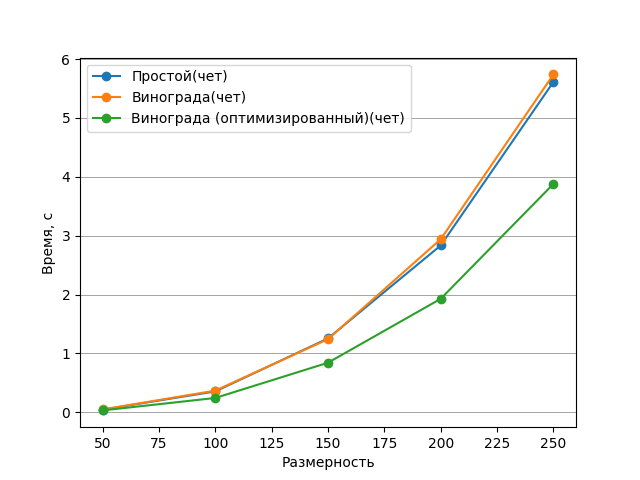
\includegraphics[scale=0.95]{imgs/1.png}
	\caption{Зависимость времени работы реализаций алгоритмов от чётной размерности квадратной матрицы}
	\label{img:profiling1}
\end{figure}

\begin{figure}[h!]
	\centering
	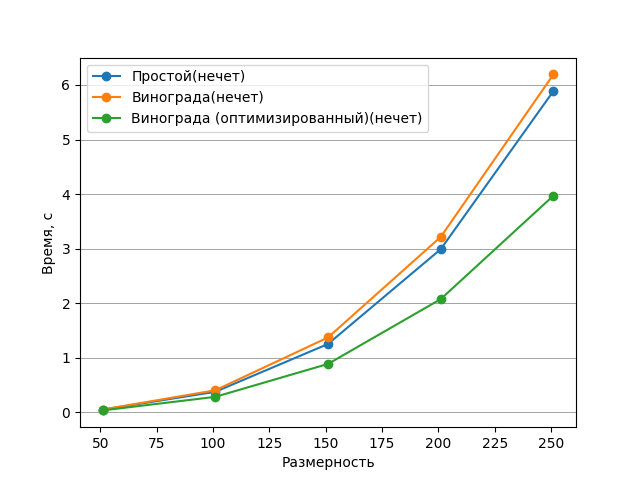
\includegraphics[scale=0.95]{imgs/2.png}
	\caption{Зависимость времени работы реализаций алгоритмов от нечётной размерности квадратной матрицы}
	\label{img:profiling2}
\end{figure}


\section{Вывод}

Оптимизированный алгоритм Винограда для перемножения матриц работает в $ \approx 1.5 $ раза \textbf{быстрее} классического 
алгоритма перемножения матриц при четных размерностях и $ \approx 1.4 $ раза -- нечетных.
В то же время, неоптимизированный алгоритм Винограда работает в $ \approx 1.03 $ раза \textbf{медленнее} классического 
алгоритма перемножения матриц при четных размерностях и $ \approx 1.07 $ раза -- нечетных.
